\documentclass[11pt,letterpaper]{article}
\usepackage[lmargin=1in,rmargin=1in,bmargin=1in,tmargin=1in]{geometry}
\usepackage{checkins}

\pgfplotsset{soldot/.style={color=black,only marks,mark=*},
		holdot/.style={color=black,fill=white,only marks,mark=*},
		compat=1.12
}

% -------------------
% Content
% -------------------
\begin{document}
\thispagestyle{title}

% 01/15
\checkin{01/15} \textit{True/False}: If $f(3)= 5$, then $\ds\lim_{x \to 3} f(x)= 5$. \pspace

\sol The statement is \textit{false}. Recall that the limit of a function (if it exists) is what the output gets `close' to as the input gets `close' to its limiting value. The fact that $f(3)= 5$ does not mean the outputs are all `close' to 5 when $x$ is `close' to 3. For instance, consider the function $f(x)$ plotted below.
	\[
	\fbox{%
	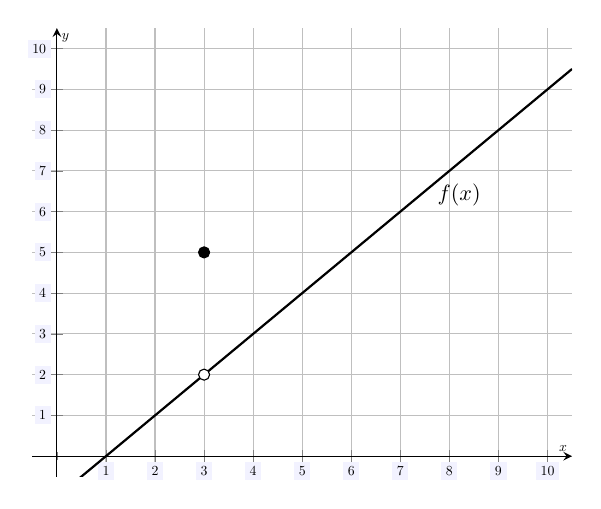
\begin{tikzpicture}[scale=1,every node/.style={scale=0.5}]
	\begin{axis}[
	grid=both,
	axis lines=middle,
	ticklabel style={fill=blue!5!white},
	xmin= -0.5, xmax=10.5,
	ymin= -0.5, ymax=10.5,
	xtick={-1,0,...,11},
	ytick={-1,0,...,11},
	minor tick = {-11,-10,...,11},
	xlabel=\(x\),ylabel=\(y\),
	samples=20]
	\node at (8.2,6.4) {\scalebox{1.6}{$f(x)$}};
	\addplot[thick, samples=5, domain= -0.5:10.5] {x - 1};
	\addplot[soldot] coordinates{(3,5)};
	\addplot[holdot] coordinates{(3,2)};
	\end{axis}
	\end{tikzpicture}
	}
	\]
Despite the fact that $f(3)= 5$, $\ds\lim_{x \to 3} f(x)= 2$ because all the outputs are `close' to 2 when the inputs are `close' to 3. \pvspace{1.3cm}



% 01/17
\checkin{01/17} \textit{True/False}: Let $f(x)$ be a function defined on all real numbers such that $\ds\lim_{x \to \pi} f(x)= 10$. Then it must be that $\ds\lim_{x \to \pi^+} f(x)= 10$. \pspace

\sol The statement is \textit{true}. Recall that the limit (if it exists) is what the output gets `close' to as the input gets `close' to its limiting value. Because $\ds\lim_{x \to \pi} f(x)= 10$, the outputs of $f(x)$ are all `close' to 10 whenever $x$ is `close' to $\pi$---no matter how $x$ is `close' to $\pi$. The right-hand limit $\ds\lim_{x \to \pi^+} f(x)$ asks what the outputs are `close' to if $x$ is `close' to $\pi$---but bigger than $\pi$. But we already know that the outputs are `close' to 10. Therefore, it must be that $\ds\lim_{x \to \pi^+} f(x)= 10$. Recall that $\ds\lim_{x \to a} f(x)= L$ if and only if $\lim_{x \to a^-} f(x)= L$ and $\lim_{x \to a^+} f(x)= L$. \pvspace{1.3cm}



% 01/22
\checkin{01/22} $\ds\lim_{x \to \infty} \left(1 + \dfrac{1}{3x} \right)^x= e^3$ \pspace

\sol The statement is \textit{false}. Recall that $\ds\lim_{x \to \infty} \left(1 + \dfrac{1}{x} \right)^x= e$. But then\dots
	\[
	\lim_{x \to \infty} \left(1 + \dfrac{1}{3x} \right)^x= \lim_{x \to \infty} \left(1 + \dfrac{1}{3x} \right)^{x \cdot 3/3}= \lim_{x \to \infty} \left[ \left(1 + \dfrac{1}{3x} \right)^{3x} \right]^{1/3}= e^{1/3}= \sqrt[3]{e}
	\] \pvspace{1.3cm}



% 01/24
\checkin{01/24} $\ds\lim_{x \to \infty} \left(1 + \dfrac{1}{x} \right)^x= \left(1 + 0\right)^\infty= 1^\infty= 1$ \pspace

\sol The statement is \textit{false}. One does obtain $1^\infty$ after na\"ively plugging in $x= \infty$. However, $\infty$ is not a number; moreover, although one might feel otherwise, it is simply need not be the case that $1^\infty= 1$. Indeed, $1^\infty$ is an indeterminant form. One could correctly recall that\dots
	\[
	\lim_{x \to \infty} \left(1 + \dfrac{1}{x} \right)^x= e
	\] \pvspace{1.3cm}



% 01/27
\checkin{01/27} The function $f(x)= \dfrac{e^x \sin(\sqrt[3]{x})}{x^2 + 6x + 9}$ is continuous on any interval which does not contain $x= -3$. \pspace

\sol The statement is \textit{true}. We know that $e^x$, $\sin x$, $\sqrt[3]{x}$, and $x^2 + 6x + 9$ are everywhere continuous. But then $\sin(\sqrt[3]{x})$ is everywhere continuous, because it is a composition of continuous functions. This makes $e^x \sin(\sqrt[3]{x})$ continuous, because it is the product of continuous functions. But then $f(x)= \dfrac{e^x \sin(\sqrt[3]{x})}{x^2 + 6x + 9}$ is continuous so long as $x^2 + 6x + 9 \neq 0$, because it would be a quotient of continuous functions. Observe that $x^2 + 6x + 9= (x + 3)^2$. Therefore, if $x^2 + 6x + 9= 0$, then $(x + 3)^2= 0$ so that $x= -3$. Therefore, $f(x)$ is continuous on any interval not containing $-3$. \pvspace{1.3cm}



% 01/29
\checkin{01/29} The limit $\ds\lim_{x \to 0} \dfrac{\sqrt{x + 9} - 3}{x}$ represents $f'(9)$, where $f(x)= \sqrt{x}$. 

\sol The statement is \textit{true}. The definition of the derivative at $x= a$ is $\ds f'(a)= \lim_{h \to 0} \dfrac{f(a + h) - f(a)}{h}$. Taking $f(x)= \sqrt{x}$ and $a= 9$, we would have $\ds f'(9)= \lim_{h \to 0} \dfrac{f(9 + h) - f(9)}{h}= \lim_{h \to 0} \dfrac{\sqrt{9 + h} - \sqrt{9}}{h}= \lim_{h \to 0} \dfrac{\sqrt{h + 9} - 3}{h}$. This is the same as the given limit with the role of $h$ and $x$ interchanged. \pvspace{1.3cm}



% 01/31
\checkin{01/31} $\dfrac{d}{dx} \, \sin(\ln x)= \cos \left( \dfrac{1}{x} \right)$ \pspace

\sol The statement is \textit{false}. We have a derivative of a composition of functions. This requires chain rule: $\frac{d}{dx}\, f \big( g(x) \big)= f' \big( g(x) \big) \cdot g'(x)$. Here, we have $f(x)= \sin x$ and $g(x)= \ln x$. The correct derivative should be\dots
	\[
	\dfrac{d}{dx} \, \sin(\ln x)= \cos(\ln x) \cdot \dfrac{1}{x}
	\]
Here, the `rule' $\frac{d}{dx} f \big( g(x) \big)= f' \big( g'(x) \big)$ has been applied, which is incorrect. \pvspace{1.3cm}



\newpage



% 02/03
\checkin{02/03} $\dfrac{d}{dx} \; x^3 \sin(x)= 3x^2 \cos x$ \pspace

\sol The statement is \textit{incorrect}. We have a derivative of a product of functions. This requires the product rule: $\frac{d}{dx} f(x) g(x)= f'(x) g(x) + f(x) g'(x)$. Here, we have $f(x)= x^3$ and $g(x)= \sin x$. The correct derivative should be\dots
	\[
	\dfrac{d}{dx}\, x^3 \sin x= 3x^2 \cdot \sin x + x^3 \cdot \cos x
	\]
Here, the `rule' $\frac{d}{dx} f(x) g(x)= f'(x) g'(x)$ has been applied, which is incorrect. \pvspace{1.3cm}



% 02/05
\checkin{02/05} If $\theta_d$ is an angle measured in degrees, then $\dfrac{d}{d\theta}\, \sin(\theta_d)= \cos(\theta_d)$. \pspace

\sol The statement is \textit{false}. This is a problem which can arise in working with derivatives with `mixed units' or especially when programming computer systems to perform the computations and one is not paying attention to the units. Trigonometric functions should be computed using radians. Even if one wishes to use degrees, the units would need to be consistent. Clearly, $\frac{d}{d\theta}$ is the derivative with respect to $\theta$---measured in radians. However, the input to the trigonometric function is in degrees. We would need to convert this input to radians by multiplying by $\frac{\pi}{180}$. But then\dots
	\[
	\dfrac{d}{d\theta} \sin(\theta_d)= \dfrac{d}{d\theta} \sin \left(\theta \cdot \dfrac{\pi}{180} \right)= \dfrac{\pi}{180} \cdot \cos \left(\theta \cdot \dfrac{\pi}{180} \right)= \dfrac{\pi}{180} \cos \left( \theta_d \right)
	\]
One can work out the derivation of $\frac{d}{d\theta} \sin \theta$ to see the reliance on radians to get a deeper---non-chain rule---reason for why this is the case. \pvspace{1.3cm}



% 02/12
\checkin{02/12} If $f'(1)= 0$ and $f''(1) < 0$, then $f(x)$ has a local minima at $x= 1$. \pspace

\sol The statement is \textit{false}. Suppose that $f(x)$ is a twice-differentiable function. If $f'(a)= 0$, then $x= a$ is a critical value for $f(x)$. By the Second Derivative Test, if $f''(a) < 0$, then $x= a$ is a local maxima. If $f''(a) > 0$, then $x= a$ is a local minima. However, if $f''(a)= 0$, then the test is inconclusive. Because $f'(1)= 0$, we know that $x= 1$ is a critical value. Because $f''(1) < 0$, then $x= 1$ is a local maxima. \pvspace{1.3cm}



% 02/14
\checkin{02/14} If $f(x)$ is differentiable at $x= a$, then the linearization of $f(x)$ at $x= a$ and the tangent line to $f(x)$ at $x= a$ are the same thing. \pspace

\sol The statement is \textit{true}. Recall that the tangent line for $f(x)$ at $x= x_0$ (if it exists) is the line $y= f(x_0) + m(x - x_0)$, where $m= f'(x_0)$. However, the linearization of $f(x)$ at $x= a$ is $\ell(x)= f(x_0) + f'(x_0) \, \big(x - x_0 \big)$. Observe that these are the same line. \pvspace{1.3cm}



\newpage



% 02/17
\checkin{02/17}  A point where $f''(x)= 0$ is called an inflection point. \pspace

\sol The statement is \textit{false}. An inflection point is a point where $f(x)$ changes concavity. Consider the function $f(x)= x^4$. Observe that $f'(x)= 4x^3$ and $f''(x)=12x^2$. We have $f''(0)= 12(0^2)= 0$. However, $f''(x)= 12x^2 \geq 0$ for all $x$. But then $f''(x)$ can never change sign, so that $f(x)$ has no points of inflection. This contradicts the assertion in the given statement. While points where $f''(x)= 0$ \textit{can} be points of inflection, they do not \textit{have} to be. \pvspace{1.3cm}



% 02/19
\checkin{02/19} $\ds\lim_{x \to 2} \dfrac{x - 2}{x^2 - 4} \stackrel{\text{L.H.}}{=} \lim_{x \to 2} \dfrac{1}{2x}= \dfrac{1}{4}$ \pspace

\sol The statement is \textit{true}. Recall that by l'H\^opital's Rule, if $\ds\lim \dfrac{f(x)}{g(x)}$ is $\dfrac{0}{0}$ or $\pm\dfrac{\infty}{\infty}$ and $\ds\lim \dfrac{f'(x)}{g'(x)}$ exists, then $\ds\lim \dfrac{f(x)}{g(x)}= \lim \dfrac{f'(x)}{g'(x)}$. Observe that `plugging in' $x= 2$ into $\dfrac{x - 2}{x^2 - 4}$, we obtain $\dfrac{0}{0}$. By l'H\^opital's Rule, we then have that this limit is the same as $\ds\lim_{x \to 2} \dfrac{1}{2x}= \dfrac{1}{2(2)}= \dfrac{1}{4}$. \pvspace{1.3cm}



% 02/21
\checkin{02/21} $\ds\lim_{x \to 1} \dfrac{4 - x}{x^2 - 1} \stackrel{\text{L.H.}}{=} \lim_{x \to 1} \dfrac{-1}{2x}= \dfrac{-1}{2(1)}= -\dfrac{1}{2}$ \pspace

\sol The statement is \textit{false}. Recall that by l'H\^opital's Rule, if $\ds\lim \dfrac{f(x)}{g(x)}$ is $\dfrac{0}{0}$ or $\pm\dfrac{\infty}{\infty}$ and $\ds\lim \dfrac{f'(x)}{g'(x)}$ exists, then $\ds\lim \dfrac{f(x)}{g(x)}= \lim \dfrac{f'(x)}{g'(x)}$. However, `plugging in' $x= 1$, we obtain $\frac{3}{0}$, which is neither of these forms. In fact, $\ds\lim_{x \to 1} \dfrac{4 - x}{x^2 - 1}$ does not exist because $\ds\lim_{x \to 1^+} \dfrac{4 - x}{x^2 - 1}= -\infty$ and $\ds\lim_{x \to 1^+} \dfrac{4 - x}{x^2 - 1}= \infty$. \pvspace{1.3cm}



% 02/24
\checkin{02/24} Implicitly differentiating $4x + y^2 + e^{xy}= y$ yields $4 + 2y + e^{xy} \cdot y + y' = y'$. \pspace

\sol The statement is \textit{false}. Recall that when implicitly differentiating $y$ with respect to $x$, we have $1 \cdot \dfrac{dy}{dx}= y'$. Therefore, we have\dots
	\[
	\begin{gathered}
	4x + y^2 + e^{xy}= y \\[0.2cm]
	\dfrac{d}{dx} \, \left(4x + y^2 + e^{xy} \right)= \dfrac{d}{dx} \, y \\[0.2cm]
	4 + 2y \cdot \dfrac{dy}{dx} + e^{xy} \cdot \left( 1 \cdot y + x \cdot \dfrac{dy}{dx} \right)= \dfrac{dy}{dx} \\[0.2cm]
	4 + 2y \cdot y' + e^{xy} \cdot \left( y + x y' \right)= y'
	\end{gathered}
	\]



\newpage



% 02/26
\checkin{02/26} If the radius of a sphere is decreasing at a rate of 1 meter per minute and is currently 2~m across, the rate of change of the volume of the sphere is $16\pi$. \pspace

\sol The statement is \textit{false}. Recall that the volume of a sphere is $V= \frac{4}{3} \,\pi r^3$. Because the sphere is 2~m across, the diameter is 2~m, i.e. the radius is $r= 1$~m. We know that the radius of the sphere is decreasing at a rate of 1~m per minute, i.e. $\frac{dr}{dt}= -1$. But then\dots
	\[
	\begin{gathered}
	V= \dfrac{4}{3} \,\pi r^3 \\
	\dfrac{d}{dt}\, V= \dfrac{d}{dt} \, \left( \dfrac{4}{3} \,\pi r^3 \right) \\
	\dfrac{dV}{dt}= 4\pi r^2 \cdot \dfrac{dr}{dt} \\
	\dfrac{dV}{dt}= 4\pi (1^2) \cdot -1 \\
	\dfrac{dV}{dt}= -4\pi
	\end{gathered}
	\]
Therefore, the volume of the sphere is decreasing at $4\pi$~m$^3$ per minute. The given answer must be incorrect as the rate of change of the volume of the sphere is positive---whereas we know the volume must be decreasing. The given answer used $r= 2$ rather than the correct value $r= 1$. \pvspace{1.3cm}



% 03/03
\checkin{03/03} If one is optimizing a function $f(x)$ on an interval $[a, b]$, if there are not critical values, then $f(x)$ has no absolute maximum or minimum on $[a, b]$. \pspace

\sol The statement is \textit{false}. Consider the function $f(x)= x$ on the interval $[-1, 1]$. Because $f'(x)= 1 \neq 0$, $f(x)$ has no critical values. However, observe that $f'(x)= 1 > 0$, so that $f(x)$ is increasing. Therefore, the smallest value for $f(x)$ must be at $x= -1$ and the largest value must be at $x= 1$. This shows that $f(-1)= -1$ is the absolute minimum for $f(x)$ on $[-1, 1]$ and $f(1)= 1$ is the absolute maximum for $f(x)$ on $[-1, 1]$. \pvspace{1.3cm}



% 03/05
\checkin{03/05} If $f'(x)$ is increasing, then $f(x)$ is convex. \pspace

\sol The statement is \textit{true}. We assume that $f''(x)$ exists. Because $f'(x)$ is increasing, we know that its derivative is positive. But $\frac{d}{dx} \,f'(x)= f''(x)$. But then $f''(x) > 0$. Because $f''(x) > 0$, we know that $f(x)$ is concave up, i.e. $f(x)$ is convex. \pvspace{1.3cm}



% 03/19
\checkin{03/19} Let $p(x)$ be an odd degree polynomial. Because $p(x)$ is everywhere continuous and $\ds\lim_{x \to \pm \infty} p(x)= \pm \infty$, by the Intermediate Value Theorem, it must be that $p(x)$ has a real root. That is, every odd degree polynomial has a real root. \pspace

\sol The statement is \textit{true}. A polynomial is everywhere continuous, so that the Intermediate Value Theorem applies to $p(x)$. If $p(x)$ has odd degree, then either $\ds\lim_{x \to \infty} p(x)= \infty$ and $\ds\lim_{x \to -\infty} p(x)= -\infty$ or $\ds\lim_{x \to \infty} p(x)= -\infty$ and $\ds\lim_{x \to -\infty} p(x)= \infty$. In either case, by the Intermediate Value Theorem, there must be an $x_0 \in (-\infty, \infty)$ such that $p(x_0)= 0$. But then $p(x)$ has a root. \pvspace{1.3cm}



% 03/21
\checkin{03/21} Starting from a stop, if you drive 250 miles in 5~hours, there had to have been a time when you drove 30~mph. \pspace

\sol The statement is \textit{true}. We assume that one's position in time, $p(t)$, is continuous and differentiable---in fact, continuously differentiable. [This should logically be the case.] Therefore, $p(t)$ is continuous on $[0, 5]$ and differentiable on $(0, 5)$. We know that the average speed over this time period is $\frac{250}{5}= 50$~mph. By the Mean Value Theorem, there is a time between 0 and 5 hours where one's speed is 50~mph. But to accelerate to 50~mph, one had to first have traveled at 30~mph (by the Intermediate Value Theorem). \pvspace{1.3cm}



% 03/24
\checkin{03/24} $\ds\sum_{n=1}^3 n^2= 14$ \pspace

\sol The statement is \textit{true}. Recall that $\ds\sum_{n=a}^b f(n)= f(a) + f(a + 1) + \cdots + f(b)$. Therefore, we have\dots
	\[
	\sum_{n=1}^3 n^2= 1^2 + 2^2 + 3^2= 1 + 4 + 9= 14
	\] \pvspace{1.3cm}



% 03/26
\checkin{03/26} The function $\sec^2(\theta) - 5$ is an antiderivative for the function $f(\theta)= \tan(\theta)$. \pspace

\sol The statement is \textit{false}. A function $F(x)$ is an antiderivative for $f(x)$ if $F'(x)= f(x)$. Observe that $\dfrac{d}{d\theta} \big( \sec^2(\theta) - 5 \big)= 2 \sec \theta \cdot \sec \theta \tan \theta - 0= 2 \sec^2 \theta \tan \theta \neq f(\theta)$. But then $\sec^2(\theta) - 5$ cannot be an antiderivative for $f(\theta)$. In fact, the antiderivative for $f(\theta)$ is $\ln|\sec \theta| + C$, where $C$ is a constant. To see this, observe that\dots
	\[
	\dfrac{d}{d\theta} \left( \ln|\sec \theta| + C \right)= \dfrac{1}{\sec \theta} \cdot \sec \theta \tan \theta + 0= \tan \theta
	\] \pvspace{1.3cm}
























\end{document}